%% Two column figure below
\begin{figure*}[htbp]
%% Size
\centerline{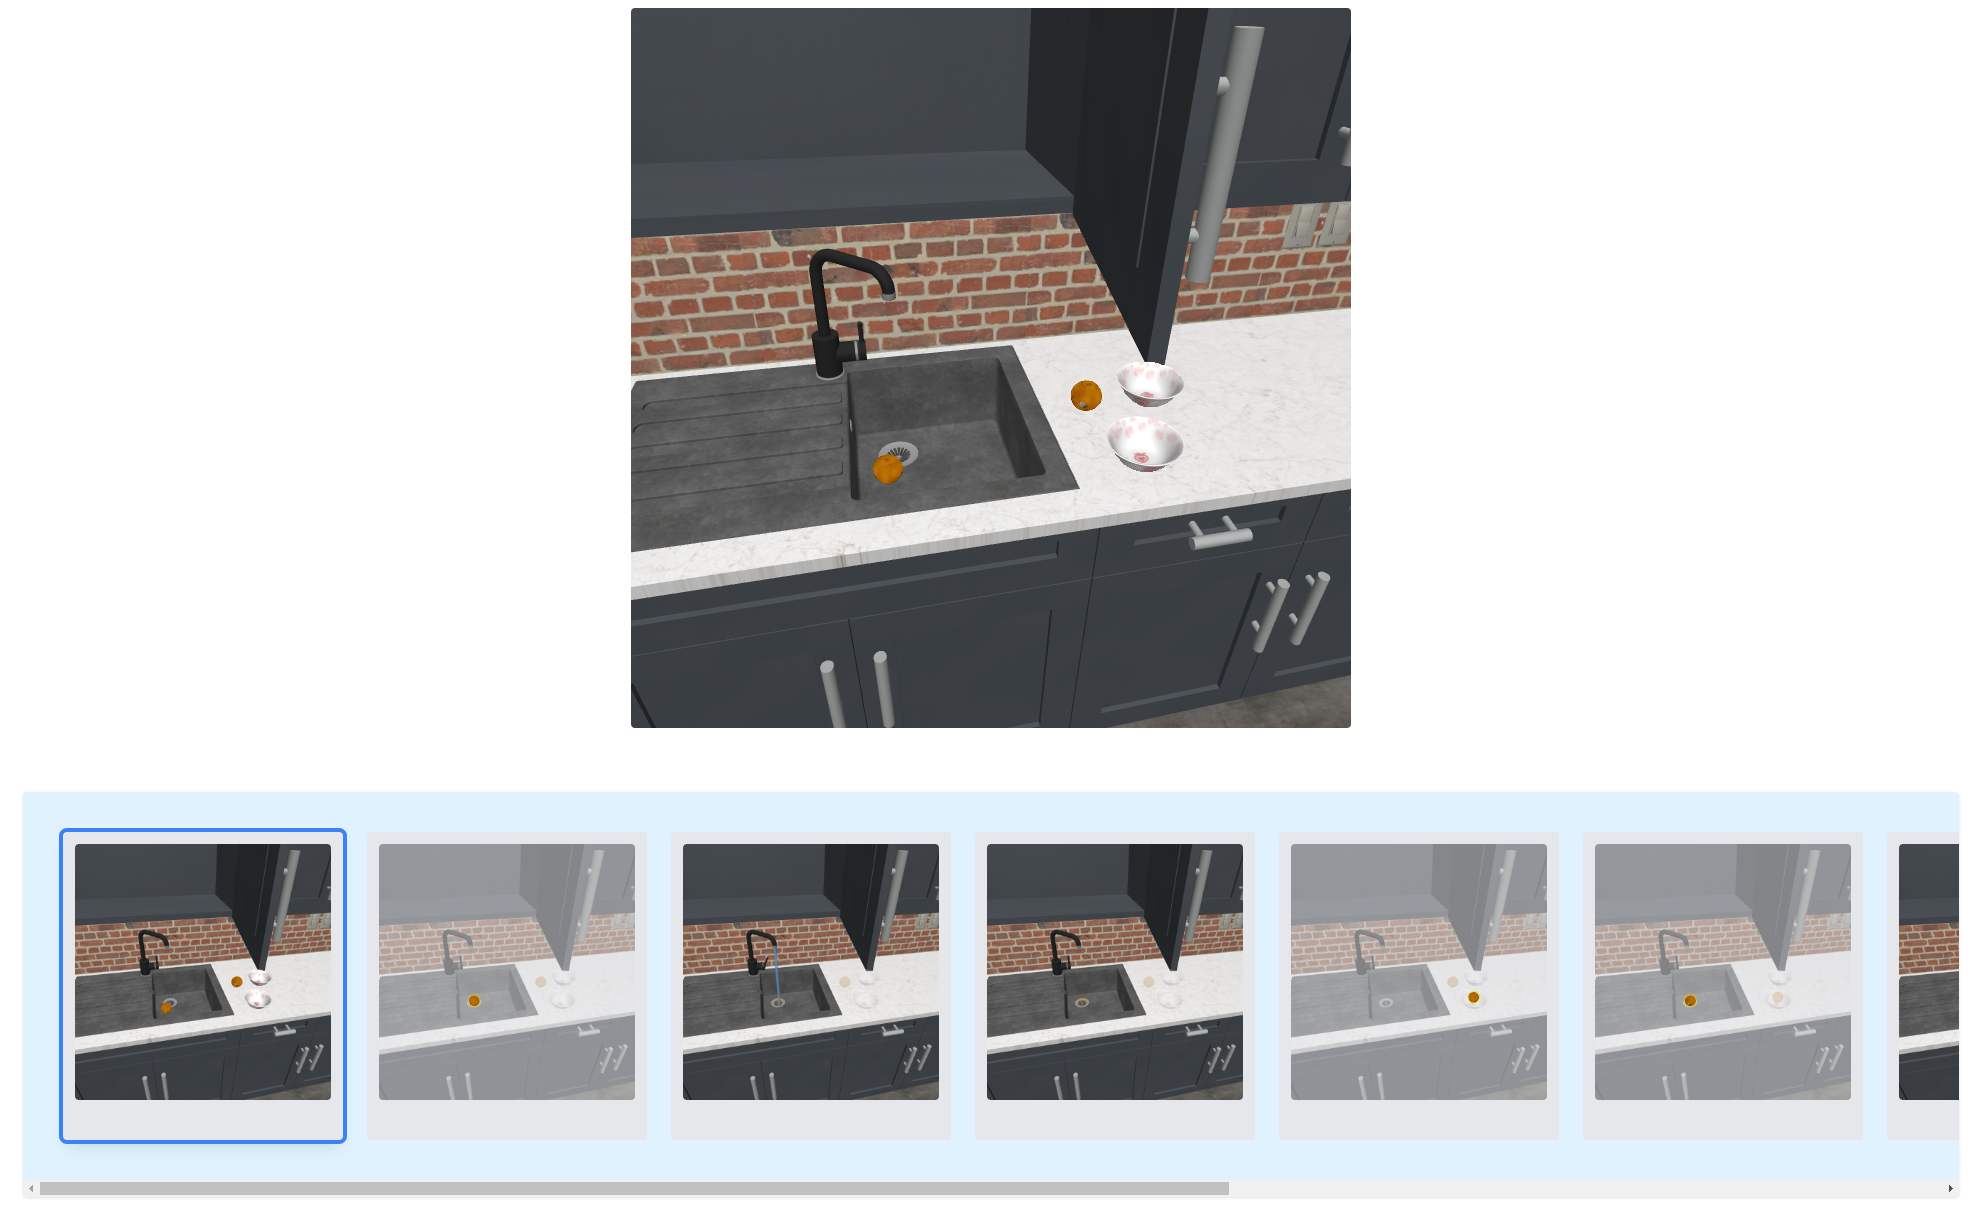
\includegraphics[width=0.8\textwidth]{figures/Interface.png}}
\caption{\projname's user interface, consisting of an editor (top) and a timeline (bottom). The editor allows users to manipulate objects and fixtures in the environment, while the timeline displays the current state of the environment and the desired changes.}
\label{fig:interface}
\end{figure*}

\section{Implementation}
\noindent \emph{High-level system design.} \projname consists of two key components: a back-end server that manages models to generate image representations and provide features like automatic captioning, and a user interface for viewing and editing images, enabling users to create and refine robot instructions through image manipulation. The server is realized as a Flask application that enables two-way communication between the models and the interface. The models are hosted as TCP sockets on workstations within the local network and communicate with the Flask server to respond to requests from the interface. The user interface is built using ReactJS. 

%% Python (Flask) + ZMQ + ReactJS

\subsection{Representing the User's Environment} 
\projname creates an initial representation of the user's environment by extracting information about the objects and fixtures present.

\noindent \emph{Background image generation.} Using the knowledge about the initial world state and possible states that each fixture can take, all possible combinations of fixture states are generated. Then, 
images representing the \textit{background} image pertaining to each possible state in the user's environment are generated. These images can be generated using a variety of methods. Specific to the simulation environment, we generate images by using LLMs to write code via to modify the state of individual fixtures that represent a given state. We envision that this could be possible in the future given that many existing applications of robots assume the existence of digital twins~\mk{CITE}. However, \projname can also generate images representing a state change based on a language instruction in the absence of a simulation environment, made possible by fine-tuning diffusion models~\cite{brooks2023instructpix2pix, black2023zero}. At the end of this process, \projname creates a background image for all possible states, and sets the background image to the one that represents the current state.

\subsection{Enabling user manipulation of images}
\noindent \emph{Generating interactable objects and fixtures.} In order to enable the direct manipulation of images, \projname begins by detecting items of interest. The items of interest can be provided as list of objects and fixtures (e.g., such as those provided by Robocasa). Or, \projname can take the current background image representing the world state state to generate the items of interest. Next, \projname generates bounding boxes for any detected items using an open vocabulary object detector, OWLv2~\cite{minderer2024scaling}. Then, information about the detected objects (not fixtures) are passed to a segmentation model, Segment Anything (SAM~\cite{kirillov2023segment}), to generate masks that can be manipulated by the user. In simulation, the objects can be hidden when generating the background image so there is no white space and direct manipulation is possible at this stage. However, for real-world tasks where objects are usually in front of the background, manipulating them can leave white space behind. Hence, \projname performs an inpainting step to eliminate white spaces behind the objects before the user manipulates them~\cite{suvorov2022resolution}. 

\noindent \emph{User manipulation of objects and fixtures through the editor.} After processing the initial world state, the background image, generated masks, and bounding boxes for the fixtures are sent to user interface and rendered as a an SVG image inside a step. When the user clicks the initial step, the underlying representation is rendered inside an image editing application (\mk{CITE website}). The editor enables simple interactions such as the selection, deselection, and manipulating individual objects. When the user performs direct manipulations on one or more objects, the system creates a new step by copying the representation of the previous step while updating data about any objects that moved. To enable interactable fixtures, bounding boxes containing the location of fixtures are utilized to detect mouse clicks within this region, which activates a state change. When changing state, the current state variable is updated and the corresponding background image is retrieved and utilized when creating the step.

\noindent \emph{Predicting future steps (autocomplete)}

%Before the user begins providing instructions to the robot, \projname creates this initial representation to represent all objects and fixtures that are present in the environment, and determines the initial state. We assume access to the initial state of fixtures in the environment, such as the presence and number of cabinets, drawers, and sinks. For instance, a sample initial state could 


%This step can either be performed manually by a user when introducing their robot to their home, or automatically using models. 



% Describe how we make this by enumerating states 

% Sim/Susie/GPT

% How we make masks

% How we make interactable regions
